\documentclass[11pt,a4paper,notitlepage]{report}
% Shared preamble for the raw chapter-4 write-ups under docs/report/insights/.
%
% Each experiment_N/experiment_N.tex is a standalone, compilable LaTeX report
% written BEFORE anything goes into final_report/chapters/chapter_4_*.tex.
% It uses the final report's fonts, units and macros so that passages, tables
% and figures lift into the chapter without reformatting.
%
%   \documentclass[11pt,a4paper]{report}
%   % Shared preamble for the raw chapter-4 write-ups under docs/report/insights/.
%
% Each experiment_N/experiment_N.tex is a standalone, compilable LaTeX report
% written BEFORE anything goes into final_report/chapters/chapter_4_*.tex.
% It uses the final report's fonts, units and macros so that passages, tables
% and figures lift into the chapter without reformatting.
%
%   \documentclass[11pt,a4paper]{report}
%   % Shared preamble for the raw chapter-4 write-ups under docs/report/insights/.
%
% Each experiment_N/experiment_N.tex is a standalone, compilable LaTeX report
% written BEFORE anything goes into final_report/chapters/chapter_4_*.tex.
% It uses the final report's fonts, units and macros so that passages, tables
% and figures lift into the chapter without reformatting.
%
%   \documentclass[11pt,a4paper]{report}
%   \input{../common/preamble}
%   \begin{document} ...
%
% Figures and tables are NOT copied: \graphicspath and \reporttable resolve into
% final_report/figures/ and final_report/tables/, so the raw write-up always
% shows the same artefacts as the chapter.  Compile with:  latexmk -pdf <file>

\usepackage[T1]{fontenc}
\usepackage[utf8]{inputenc}
\usepackage{mathptmx}
\usepackage[scaled=0.92]{helvet}
\usepackage{courier}
\usepackage[a4paper,left=30mm,right=20mm,top=25mm,bottom=25mm]{geometry}
\usepackage{microtype}
\usepackage{booktabs}
\usepackage{tabularx}
\usepackage{longtable}
\usepackage{array}
\usepackage{multirow}
\usepackage{amsmath}
\usepackage{amssymb}
\usepackage{ifthen}
\usepackage{siunitx}
\usepackage{graphicx}
\usepackage{placeins}
\usepackage{caption}
\usepackage{enumitem}
\usepackage[table]{xcolor}
\usepackage{rotating}
\PassOptionsToPackage{hyphens}{url}\usepackage{url}
\usepackage[hidelinks]{hyperref}
\usepackage[nameinlink,noabbrev]{cleveref}

\graphicspath{{../../final_report/}{../../final_report/figures/}}
% \reporttable{name} inputs final_report/tables/name.tex
\newcommand{\reporttable}[1]{\input{../../final_report/tables/#1}}

\newcommand{\repo}[1]{\texttt{\detokenize{#1}}}
\sisetup{detect-all,group-separator={,},range-phrase=--,range-units=single}
\DeclareSIUnit{\pixel}{px}
\DeclareSIUnit{\mebi}{Mi}
\captionsetup{font=small,labelfont=bf}
\setlist{nosep}
\setlength{\parskip}{4pt}
\setlength{\LTcapwidth}{\textwidth}

% ---- result-slot status (RENDERED here, unlike in the final report)
\definecolor{stcompleted}{HTML}{A5D6A7}
\definecolor{stpartial}{HTML}{FFF2CC}
\definecolor{stuntested}{HTML}{FFD8A8}
\definecolor{stblocked}{HTML}{FFCDD2}
\definecolor{stfailed}{HTML}{FFCDD2}
\definecolor{stplanned}{HTML}{E0E0E0}
\newcommand{\slotstatus}[2]{%
  \par\noindent\fcolorbox{black!40}{st#1}{\parbox{\dimexpr\textwidth-2\fboxsep-2\fboxrule}{%
    \textbf{Status: #1.}\ #2}}\par\medskip}
\newcommand{\status}[1]{\textbf{#1}}

% ---- queries: RENDERED in red here so a reader sees every open concern in place
\definecolor{flagred}{HTML}{B00000}
\newcommand{\flag}[1]{\textcolor{flagred}{#1}}
\newcommand{\moved}[1]{#1}
\newenvironment{queried}[1][Questionable]%
  {\par\addvspace{0.6ex}\begingroup\color{flagred}\noindent
   \textbf{[#1]}\ \ignorespaces}%
  {\par\endgroup\addvspace{0.6ex}}

% ---- per-block performance marks (section 4.5 diagrams)
\definecolor{perfgood}{HTML}{A5D6A7}
\definecolor{perfpoor}{HTML}{FFCDD2}
\definecolor{perfnoeffect}{HTML}{D9EAF7}
\definecolor{perfnone}{HTML}{FFF2CC}
\newcommand{\perfmark}[1]{%
  \ifthenelse{\equal{#1}{good}}{\colorbox{perfgood}{\scriptsize good}}{%
  \ifthenelse{\equal{#1}{poor}}{\colorbox{perfpoor}{\scriptsize poor}}{%
  \ifthenelse{\equal{#1}{noeffect}}{\colorbox{perfnoeffect}{\scriptsize no effect}}{%
  \colorbox{perfnone}{\scriptsize no claim}}}}}

%   \begin{document} ...
%
% Figures and tables are NOT copied: \graphicspath and \reporttable resolve into
% final_report/figures/ and final_report/tables/, so the raw write-up always
% shows the same artefacts as the chapter.  Compile with:  latexmk -pdf <file>

\usepackage[T1]{fontenc}
\usepackage[utf8]{inputenc}
\usepackage{mathptmx}
\usepackage[scaled=0.92]{helvet}
\usepackage{courier}
\usepackage[a4paper,left=30mm,right=20mm,top=25mm,bottom=25mm]{geometry}
\usepackage{microtype}
\usepackage{booktabs}
\usepackage{tabularx}
\usepackage{longtable}
\usepackage{array}
\usepackage{multirow}
\usepackage{amsmath}
\usepackage{amssymb}
\usepackage{ifthen}
\usepackage{siunitx}
\usepackage{graphicx}
\usepackage{placeins}
\usepackage{caption}
\usepackage{enumitem}
\usepackage[table]{xcolor}
\usepackage{rotating}
\PassOptionsToPackage{hyphens}{url}\usepackage{url}
\usepackage[hidelinks]{hyperref}
\usepackage[nameinlink,noabbrev]{cleveref}

\graphicspath{{../../final_report/}{../../final_report/figures/}}
% \reporttable{name} inputs final_report/tables/name.tex
\newcommand{\reporttable}[1]{\input{../../final_report/tables/#1}}

\newcommand{\repo}[1]{\texttt{\detokenize{#1}}}
\sisetup{detect-all,group-separator={,},range-phrase=--,range-units=single}
\DeclareSIUnit{\pixel}{px}
\DeclareSIUnit{\mebi}{Mi}
\captionsetup{font=small,labelfont=bf}
\setlist{nosep}
\setlength{\parskip}{4pt}
\setlength{\LTcapwidth}{\textwidth}

% ---- result-slot status (RENDERED here, unlike in the final report)
\definecolor{stcompleted}{HTML}{A5D6A7}
\definecolor{stpartial}{HTML}{FFF2CC}
\definecolor{stuntested}{HTML}{FFD8A8}
\definecolor{stblocked}{HTML}{FFCDD2}
\definecolor{stfailed}{HTML}{FFCDD2}
\definecolor{stplanned}{HTML}{E0E0E0}
\newcommand{\slotstatus}[2]{%
  \par\noindent\fcolorbox{black!40}{st#1}{\parbox{\dimexpr\textwidth-2\fboxsep-2\fboxrule}{%
    \textbf{Status: #1.}\ #2}}\par\medskip}
\newcommand{\status}[1]{\textbf{#1}}

% ---- queries: RENDERED in red here so a reader sees every open concern in place
\definecolor{flagred}{HTML}{B00000}
\newcommand{\flag}[1]{\textcolor{flagred}{#1}}
\newcommand{\moved}[1]{#1}
\newenvironment{queried}[1][Questionable]%
  {\par\addvspace{0.6ex}\begingroup\color{flagred}\noindent
   \textbf{[#1]}\ \ignorespaces}%
  {\par\endgroup\addvspace{0.6ex}}

% ---- per-block performance marks (section 4.5 diagrams)
\definecolor{perfgood}{HTML}{A5D6A7}
\definecolor{perfpoor}{HTML}{FFCDD2}
\definecolor{perfnoeffect}{HTML}{D9EAF7}
\definecolor{perfnone}{HTML}{FFF2CC}
\newcommand{\perfmark}[1]{%
  \ifthenelse{\equal{#1}{good}}{\colorbox{perfgood}{\scriptsize good}}{%
  \ifthenelse{\equal{#1}{poor}}{\colorbox{perfpoor}{\scriptsize poor}}{%
  \ifthenelse{\equal{#1}{noeffect}}{\colorbox{perfnoeffect}{\scriptsize no effect}}{%
  \colorbox{perfnone}{\scriptsize no claim}}}}}

%   \begin{document} ...
%
% Figures and tables are NOT copied: \graphicspath and \reporttable resolve into
% final_report/figures/ and final_report/tables/, so the raw write-up always
% shows the same artefacts as the chapter.  Compile with:  latexmk -pdf <file>

\usepackage[T1]{fontenc}
\usepackage[utf8]{inputenc}
\usepackage{mathptmx}
\usepackage[scaled=0.92]{helvet}
\usepackage{courier}
\usepackage[a4paper,left=30mm,right=20mm,top=25mm,bottom=25mm]{geometry}
\usepackage{microtype}
\usepackage{booktabs}
\usepackage{tabularx}
\usepackage{longtable}
\usepackage{array}
\usepackage{multirow}
\usepackage{amsmath}
\usepackage{amssymb}
\usepackage{ifthen}
\usepackage{siunitx}
\usepackage{graphicx}
\usepackage{placeins}
\usepackage{caption}
\usepackage{enumitem}
\usepackage[table]{xcolor}
\usepackage{rotating}
\PassOptionsToPackage{hyphens}{url}\usepackage{url}
\usepackage[hidelinks]{hyperref}
\usepackage[nameinlink,noabbrev]{cleveref}

\graphicspath{{../../final_report/}{../../final_report/figures/}}
% \reporttable{name} inputs final_report/tables/name.tex
\newcommand{\reporttable}[1]{\input{../../final_report/tables/#1}}

\newcommand{\repo}[1]{\texttt{\detokenize{#1}}}
\sisetup{detect-all,group-separator={,},range-phrase=--,range-units=single}
\DeclareSIUnit{\pixel}{px}
\DeclareSIUnit{\mebi}{Mi}
\captionsetup{font=small,labelfont=bf}
\setlist{nosep}
\setlength{\parskip}{4pt}
\setlength{\LTcapwidth}{\textwidth}

% ---- result-slot status (RENDERED here, unlike in the final report)
\definecolor{stcompleted}{HTML}{A5D6A7}
\definecolor{stpartial}{HTML}{FFF2CC}
\definecolor{stuntested}{HTML}{FFD8A8}
\definecolor{stblocked}{HTML}{FFCDD2}
\definecolor{stfailed}{HTML}{FFCDD2}
\definecolor{stplanned}{HTML}{E0E0E0}
\newcommand{\slotstatus}[2]{%
  \par\noindent\fcolorbox{black!40}{st#1}{\parbox{\dimexpr\textwidth-2\fboxsep-2\fboxrule}{%
    \textbf{Status: #1.}\ #2}}\par\medskip}
\newcommand{\status}[1]{\textbf{#1}}

% ---- queries: RENDERED in red here so a reader sees every open concern in place
\definecolor{flagred}{HTML}{B00000}
\newcommand{\flag}[1]{\textcolor{flagred}{#1}}
\newcommand{\moved}[1]{#1}
\newenvironment{queried}[1][Questionable]%
  {\par\addvspace{0.6ex}\begingroup\color{flagred}\noindent
   \textbf{[#1]}\ \ignorespaces}%
  {\par\endgroup\addvspace{0.6ex}}

% ---- per-block performance marks (section 4.5 diagrams)
\definecolor{perfgood}{HTML}{A5D6A7}
\definecolor{perfpoor}{HTML}{FFCDD2}
\definecolor{perfnoeffect}{HTML}{D9EAF7}
\definecolor{perfnone}{HTML}{FFF2CC}
\newcommand{\perfmark}[1]{%
  \ifthenelse{\equal{#1}{good}}{\colorbox{perfgood}{\scriptsize good}}{%
  \ifthenelse{\equal{#1}{poor}}{\colorbox{perfpoor}{\scriptsize poor}}{%
  \ifthenelse{\equal{#1}{noeffect}}{\colorbox{perfnoeffect}{\scriptsize no effect}}{%
  \colorbox{perfnone}{\scriptsize no claim}}}}}

\renewcommand{\bibname}{References}
% Paths break at / . _ here (url's \path), where the shared \repo (texttt +
% detokenize) cannot: this note cites long run directories inside table cells.
\urlstyle{tt}
\renewcommand*\UrlBreaks{\do\/\do\_\do\.\do\-}
\renewcommand{\repo}[1]{\path{#1}}
\newcommand{\repoc}[1]{\texttt{\detokenize{#1}}}   % for captions (moving arguments)
\setcounter{chapter}{3}
\renewcommand{\thesection}{\arabic{section}}
\renewcommand{\thefigure}{R.\arabic{figure}}
\renewcommand{\thetable}{R.\arabic{table}}
\title{RTAB-Map Back End: Simulation and Real-World Configuration\\
       \large Engineering note for Chapter~3 (implemented system) and Experiment~4 (dense map)}
\author{Bolton Athit Davies}
\date{Reporting cutoff: 2 November 2026}
\begin{document}
\maketitle

\noindent\textbf{Purpose of this document.} RTAB-Map \cite{labbe2019} is the
mapping back end of Pipeline~2. It runs behind a front end that supplies the
pose, and it is configured differently in the two domains because the two
camera rigs differ. This note records both configurations as they are
implemented at the cutoff, the measurements each setting rests on, and the
validity checks that decide whether a real-rig map can be trusted. Every number
traces to a file named in \cref{sec:rtab-rules}. Experiment~4 results are not
restated here beyond the figures needed to justify a setting.

\slotstatus{completed}{\textbf{Simulation configuration.} Construct, extend and
localize modes are implemented and exercised; the tiny-map and realistic-world
databases were built and scored against ground truth (Experiment~4,
simulation slot). The configuration has been stable since 9~September 2026
apart from the \repo{loop_closure} switch added on 26~October.}

\slotstatus{partial}{\textbf{Real-world configuration.} The fisheye rig is
rectified in the shim and two recordings (28 and 31~October) produced
databases, so the chain runs end to end. Three items are open: the IMU height
above the floor is \flag{not measured} (the base frame uses a
\SI{0.30}{\metre} placeholder); the 31~October recording needs a chequerboard
calibration of the moved mount (a self-calibration from the bag stands in);
and no independent ground truth exists for the real site, so no map-quality
metric can be reported for either database.}

% =====================================================================
\section{What is common to both domains}
\label{sec:rtab-common}

RTAB-Map never receives odometry as a topic. It takes the pose from TF, so the
front end is whichever node publishes the \repo{odom_frame} to
\repo{body_frame} transform. Swapping ORB-SLAM3 \cite{campos2021} for
VINS-Fusion \cite{qin2018vins} changes nothing in the back end. The
measurement behind this choice is in \cref{tab:rtab-measured}: with odometry
on a topic the five-way synchroniser evicted the pose before its stereo pair
arrived and the run kept three nodes; from TF the same bag gave 28.

Both domains run the same five packages of the wrapper fork
(\repo{rtabmap_msgs}, \repo{rtabmap_conversions}, \repo{rtabmap_util},
\repo{rtabmap_sync}, \repo{rtabmap_slam}) against the apt core library
\repo{ros-humble-rtabmap} 0.23.7. The fork is pinned to upstream
\repo{2eef2b3}, the newest ROS~2 commit that builds against 0.23.7;
RTAB-Map's own visual odometry package is not built because the front ends
replace it.

Both domains share one launch file, \repo{rtabmap_ros/rtab_sim.launch.py},
and one input shim, \repo{rtabmap_ros/rtab_camera_shim.py}. The shim
manufactures what the bags lack: a decoded stereo pair, both
\repo{camera_info} messages, and the static transforms from the body frame to
the two optical frames, all derived from the VINS configuration directory so
the two pipelines read one calibration. A \repo{camera_model} switch selects
the pinhole path (simulation) or the fisheye path (real rig);
\cref{tab:rtab-shared} lists what the two paths share.

\begin{table}[htbp]
\centering
\caption{Launch and RTAB-Map settings common to both domains. Values are those
set in \repoc{rtab_sim.launch.py}; ``argument'' marks a launch argument with
its default.}
\label{tab:rtab-shared}
\small
\begin{tabular}{@{}p{4.6cm}p{3.3cm}p{7.1cm}@{}}
\toprule
Setting & Value & Reason \\
\midrule
Pose source & TF \repo{odom_frame}$\to$\repo{body_frame} & see \cref{tab:rtab-measured} \\
\repo{approx_sync} / \repo{sync_queue_size} & true / 30 & four image topics stamped identically by the shim \\
\repo{topic_queue_size} & 200 & raised from 10 for the odometry-topic layout; no longer load-bearing \\
\repo{wait_for_transform} (argument) & \SI{5}{\second} & front-end lag under replay; with a replayed trajectory it is never waited on \\
\repo{Stereo/DenseStrategy} & 1 (SGBM \cite{hirschmuller2008}) & block matching returned confident garbage on blank floor and walls \\
\repo{Mem/UseOdomGravity} & true & no IMU reaches RTAB-Map; the front end is gravity-aligned (33 gravity links vs 0) \\
\repo{RGBD/OptimizeMaxError} (argument) & 3.0 & upstream default; see \cref{tab:rtab-measured} for its effect with VINS \\
\repo{Grid/RayTracing} & true & the floor yields no stereo points, so free space exists only by ray tracing \\
\repo{Grid/NormalsSegmentation} & false & height-based ground split \\
\repo{Grid/MaxGroundHeight} (\repo{ground_height}) & 0.1 & measured in \repo{base_frame} \\
\repo{Grid/MaxObstacleHeight} & \SI{2.0}{\metre} & ceiling of the obstacle band \\
{\footnotesize\repo{Grid/NoiseFilteringRadius}\newline \repo{Grid/NoiseFilteringMinNeighbors}} & 0.1, 5 & drops isolated speckle \\
\repo{Grid/RangeMax} (\repo{grid_range_max}) & 10.0 & simulation default after the range sweep \\
\repo{Rtabmap/DetectionRate} (\repo{detection_rate}) & \SI{1.0}{\hertz} & node creation rate \\
\repo{loop_closure} (argument) & true & false sets \repo{Rtabmap/LoopThr}=1.0 and \repo{RGBD/ProximityBySpace}=false, keeping visual words so the database still localises \\
\repo{mode} (argument) & construct & extend / localize switch \repo{Mem/IncrementalMemory}, \repo{Mem/InitWMWithAllNodes}, \repo{RGBD/StartAtOrigin}, \repo{RGBD/CreateOccupancyGrid} \\
Database wipe & \repo{-d} in construct only & refused in extend / localize; a non-\repo{.db} path is resolved to \repo{<path>/rtabmap.db} \\
Bag replay & without \repo{--clock} & the bags record \repo{/clock}; a second clock cleared the TF buffer 1724 times \\
\bottomrule
\end{tabular}
\end{table}

\begin{table}[htbp]
\centering
\caption{Settings that were measured rather than assumed. Each row is an A/B on
one bag with only the named setting changed (engineering record, Sections~6,
6c and 7).}
\label{tab:rtab-measured}
\small
\begin{tabular}{@{}p{3.8cm}p{2.8cm}p{4.9cm}p{3.2cm}@{}}
\toprule
Setting & Condition & Result & Bag \\
\midrule
Pose from odometry topic & 5-topic sync, \SI{40}{\hertz} odom & 7 starvation warnings, 3 nodes, 1 closure & \repo{static_dataset_loop} \\
Pose from TF & 4-topic sync & 0 warnings, 28 nodes, 2 closures & same \\
\repo{Mem/UseOdomGravity} false & default & 0 gravity links, map tilted & \repo{dataset_static} \\
\repo{Mem/UseOdomGravity} true & & 33 gravity links (one per node), level & same \\
Extrinsic misread by \repo{cv2.FileStorage} & camera pitched \SI{34}{\degree} & 9 closures; grid precision \SI{42}{\percent}, Chamfer p95 \SI{1.85}{\metre} & \repo{dataset_static_tiny_repeat} \\
Extrinsic parsed from text, rigidity-checked & & 72 closures; precision \SI{91}{\percent}, p95 \SI{0.35}{\metre} & same \\
\repo{RGBD/OptimizeMaxError} 3.0, VINS odometry & drift \SIrange{0.1}{0.2}{\metre} & 36 closures detected, 0 accepted & same \\
\repo{RGBD/OptimizeMaxError} 10.0, VINS odometry & & 36 accepted & same \\
\repo{RGBD/OptimizeMaxError} 3.0, ground-truth odometry & & 72 accepted & same \\
\bottomrule
\end{tabular}
\end{table}

% =====================================================================
\section{Simulation configuration}
\label{sec:rtab-sim}

\subsection{Sensor model}

The simulated camera is an ideal pinhole, so the shim publishes the raw
frames as \repo{image_rect} with no rectification and exits if any distortion
term in the calibration is non-zero. \Cref{tab:rtab-sim-sensor} gives the
values it derives from \repo{vins_fusion_ros2/config/wil_sim/}. Both frames
are stamped with the left frame's time, as the ORB-SLAM3 node does, so the two
pipelines consume the same pair.

\begin{table}[htbp]
\centering
\caption{Simulation stereo model as published by the shim
(\repoc{camera_model:=pinhole}).}
\label{tab:rtab-sim-sensor}
\small
\begin{tabular}{@{}p{3.4cm}p{12.1cm}@{}}
\toprule
Quantity & Value \\
\midrule
Resolution & \num{1280}$\times$\num{720} \\
$f_x = f_y$; $c_x, c_y$ & 640.0; 640.0, 360.0 \\
Distortion & all terms 0 \\
Left / right camera & cam0 / cam1 (cam0 at body $y=+0.0936$; disparity check +11.9\,px) \\
Baseline $B$; $f_x B$ & \SI{93.6}{\milli\metre}; \SI{59.9}{\pixel\metre} \\
Body frame & IMU, forward-left-up; body$\to$optical quaternion $(0.5,-0.5,0.5,-0.5)$ \\
Published rate & \SI{4}{\hertz} on the message stamp (\SI{3.2}{\hertz} achieved) \\
\bottomrule
\end{tabular}
\end{table}

\subsection{Mapping run as used for the realistic worlds}

The simulation mapping runs use the ORB-SLAM3 front end with its own loop
closing off, so RTAB-Map is the only component that may close loops.
\Cref{tab:rtab-sim-run} lists the arguments of the command in use against the
launch defaults. \repo{ground_height} is \num{0.29} rather than the default
\num{0.1} because the ORB-SLAM3 node publishes the pose of \repo{base_footprint},
which sits \SI{0.192}{\metre} below the IMU body the default was measured for.

\begin{table}[htbp]
\centering
\caption{Simulation mapping command (realistic worlds, ORB-SLAM3 front end)
against the launch defaults.}
\label{tab:rtab-sim-run}
\small
\begin{tabular}{@{}p{3.2cm}p{3.4cm}p{1.8cm}p{6.2cm}@{}}
\toprule
Argument & Used & Default & Note \\
\midrule
\repo{mode} & construct & construct & \\
\repo{odom_frame} / \repo{body_frame} & \repo{orbslam3_world} / \repo{base_footprint} & \repo{world} / \repo{body} & defaults are the VINS frame names \\
\repo{ground_height} & 0.29 & 0.1 & base\_footprint instead of IMU body \\
\repo{grid_range_max} & 8.0 & 10.0 & $f_xB = 59.9$: 1\,px error is \SI{1.1}{\metre} at \SI{8}{\metre} \\
\repo{detection_rate} & 4.0 & 1.0 & keyframe density sets how often a cell is observed \\
\repo{shim_rate} & 4.0 & 4.0 & \\
\repo{loop_closure} & false & true & closure-free map; closures scored separately \\
\repo{rviz} & true & false & stock displays, no RTAB-Map plugins built \\
ORB \repo{loopClosing} (config) & 0 & -- & A/B on the mapping bags: ATE \num{2.01}$\to$\SI{0.07}{\metre} and \num{8.82}$\to$\SI{0.10}{\metre} \\
Bag rate & \numrange{0.3}{0.5} & -- & keeps the front end's backlog below the TF window \\
\bottomrule
\end{tabular}
\end{table}

\subsection{Front-end coupling}

The front end runs in a separate terminal and only its transform is consumed.
Running VINS and RTAB-Map together from a bag failed on this laptop (VINS
diverged; mechanism not identified), so the VINS localisation levels were
measured by replaying a recorded VINS trajectory through
\repo{script/gt_tf_publisher.py} instead. The same replay route is the
standard procedure on the real rig (\cref{sec:rtab-real-passes}).

Maps built with this configuration are scored in the Experiment~4 write-up,
with their tolerances and sample counts; the scores are not restated here.

% =====================================================================
\section{Real-world configuration}
\label{sec:rtab-real}

\subsection{Sensor model and rectification}

The real rig's cameras are \SI{180}{\degree} Kannala--Brandt \cite{kannala2006}
fisheyes at \num{1920}$\times$\num{1080}, and RTAB-Map's stereo path has no
equidistant model, so the shim rectifies every pair onto a virtual pinhole
before publishing (\repo{camera_model:=fisheye}). \Cref{tab:rtab-real-sensor}
gives the model; \cref{fig:rtab-real-pair} shows a rectified pair. The
projection matrices are built by hand from \repo{hfov_deg} because OpenCV's
own estimate returned $f_x = 0$ for a lens whose corners map to infinity; only
its rectification rotations are used.

\begin{table}[htbp]
\centering
\caption{Real-rig stereo model as published by the shim
(\repoc{camera_model:=fisheye}, 28~October calibration).}
\label{tab:rtab-real-sensor}
\small
\begin{tabular}{@{}p{3.4cm}p{12.1cm}@{}}
\toprule
Quantity & Value \\
\midrule
Lens model & Kannala--Brandt; $k_1..k_4 = (-3.65\times10^{-2},\ -8.40\times10^{-4},\ 1.77\times10^{-4},\ -3.83\times10^{-4})$ \\
Native intrinsics & $f = 607.5, 609.9$; $c = (958.3, 539.8)$; cam1 reuses cam0's (one mono calibration exists) \\
Left / right camera & cam1 / cam0 (\repo{left_cam:=1}; cam1 is left since the 19~October remount) \\
Extrinsic & \repo{camera_parameters_281026}: $B = \SI{89.0}{\milli\metre}$, \SI{0.86}{\degree} \\
Virtual pinhole & \repo{hfov_deg} 110: $f_x = 672.2$, $f_x B = \SI{59.8}{\pixel\metre}$ (the simulation's budget) \\
\repo{rect_scale} 0.5 & \num{960}$\times$\num{540}, $f_x = 336.1$, $f_x B = \SI{29.9}{\pixel\metre}$ \\
Rectification rotations & \SI{1.2}{\degree} (left), \SI{1.7}{\degree} (right) \\
Published frames & \repo{cam1_rect_optical}, \repo{cam0_rect_optical}; left bgr8, right mono8 \\
\bottomrule
\end{tabular}
\end{table}

\begin{figure}[htbp]
\centering
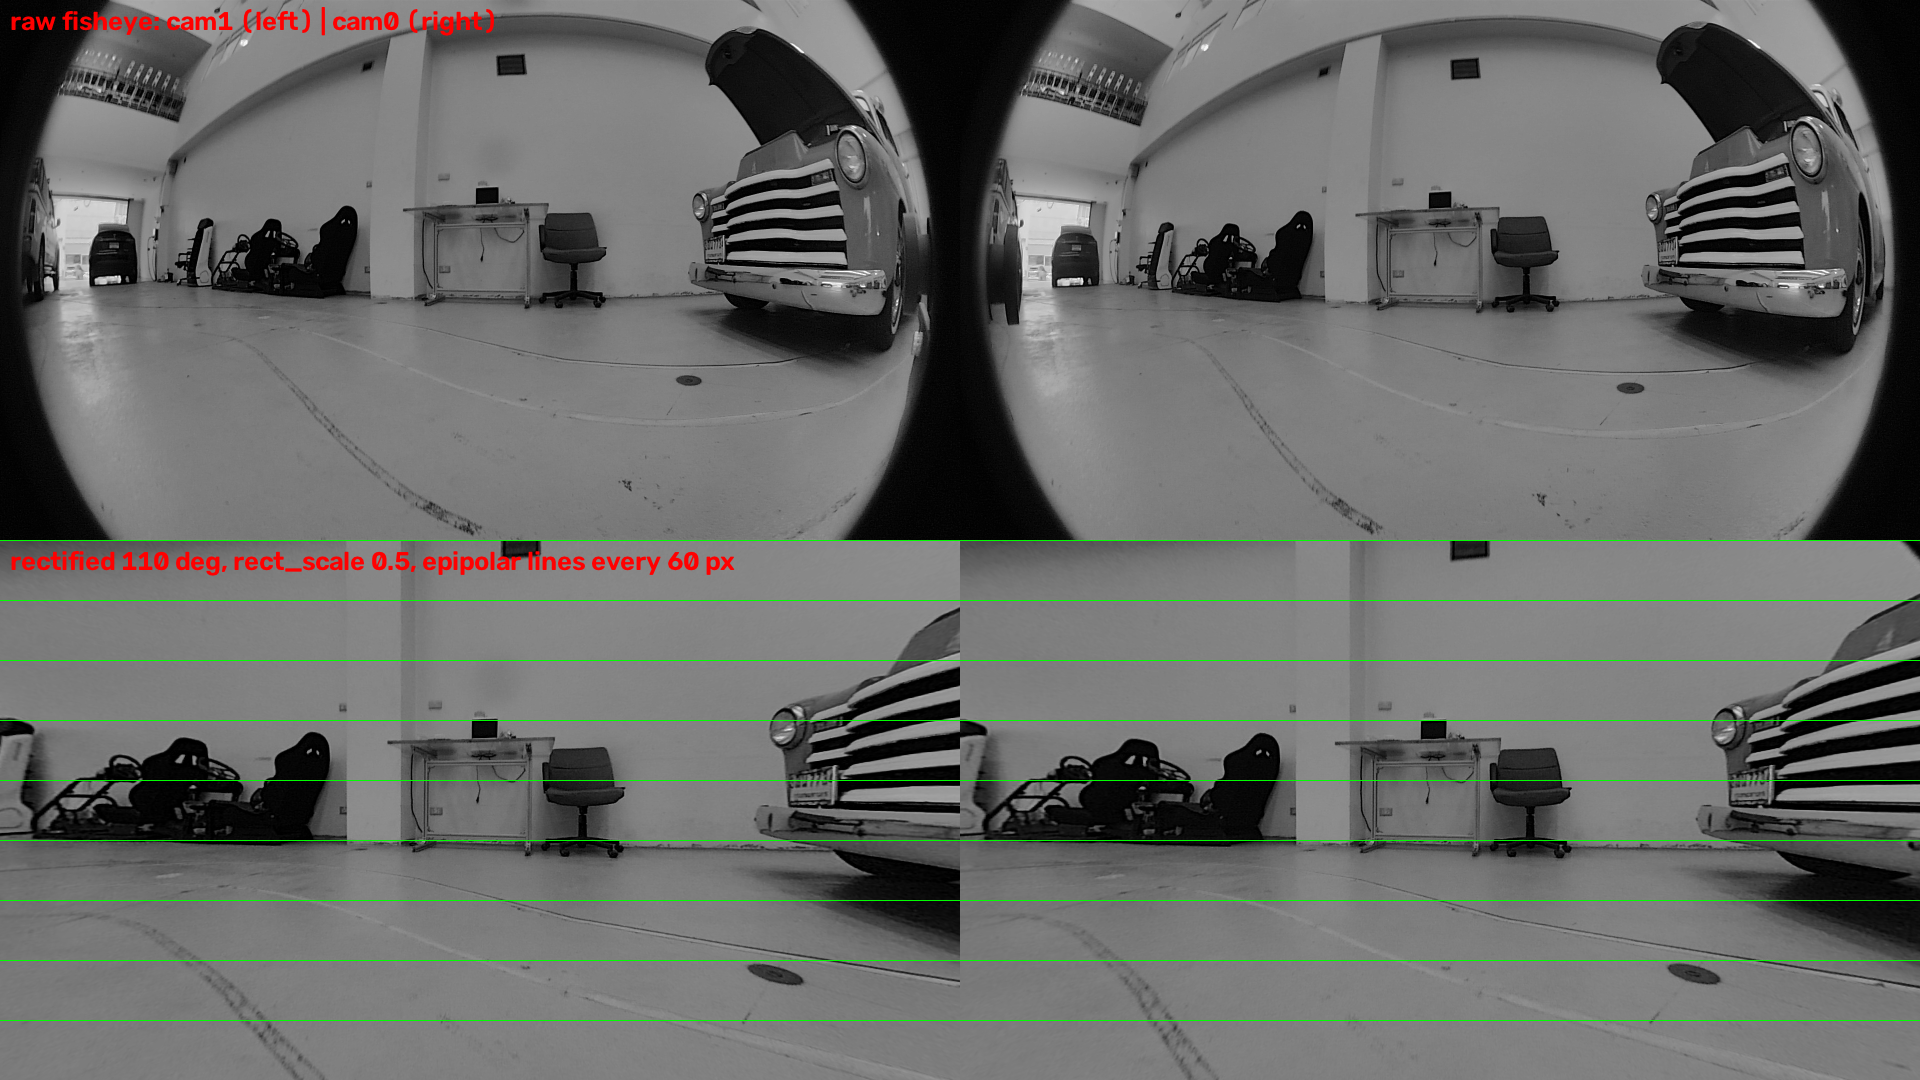
\includegraphics[width=\textwidth]{rtab/rtab_realv5_rectified_pair.png}
\caption{A realv5 pair before and after rectification (frame 1500,
\repoc{hfov_deg} 110, \repoc{rect_scale} 0.5). The table edge, chair and car
grille fall on the same horizontal lines in both halves.}
\label{fig:rtab-real-pair}
\end{figure}

Three invariants are checked at start-up, each of which failed silently at
least once while the path was built: the camera named \repo{left_cam} must have
the other camera at $+x$ in its optical frame; the two published rectified
frames must form a canonical pair, right at $(B,0,0)$ with identity rotation,
to \num{e-6}; and the extrinsic is parsed from the configuration text with
comments stripped, because the real-rig file keeps five retired calibrations
as commented blocks under the same key and the first match was a pre-remount
value.

\Cref{tab:rtab-hfov} is the field-of-view trade. A wider virtual view keeps
more of the fisheye but lowers the focal length, and the depth error per pixel
of disparity is $z^2/(f_x B)$. The default of \SI{110}{\degree} reproduces the
simulation's depth budget.

\begin{table}[htbp]
\centering
\caption{Virtual field of view against depth budget and epipolar alignment on
three realv5 frames at full resolution (cross-checked ORB matches within
\SI{2}{\pixel} of the epipolar line, positive disparity).}
\label{tab:rtab-hfov}
\small
\begin{tabular}{@{}S[table-format=3]S[table-format=3]S[table-format=2.1]S[table-format=2]@{}}
\toprule
{HFOV [\si{\degree}]} & {$f_x$ [\si{\pixel}]} & {$f_x B$ [\si{\pixel\metre}]} & {on-line matches [\si{\percent}]} \\
\midrule
90  & 960 & 85.5 & 35 \\
110 & 672 & 59.8 & 53 \\
130 & 448 & 39.9 & 69 \\
\bottomrule
\end{tabular}
\end{table}

\subsection{Frames}

\repo{imu_link}, the frame the real ORB-SLAM3 launch publishes under
\repo{orbslam3_world}, cannot be RTAB-Map's base frame. The IMU extrinsic
\repo{IMU.T_b_c1} = diag$(1,-1,-1)$ makes it x-right, y-up, z-backward, and
RTAB-Map measures ground height along the base frame's $z$. A forward-left-up
\repo{base_link} is therefore hung under it with a static transform (pitch and
yaw \SI{90}{\degree}, translation $(0,-h,0)$ with $h$ the IMU height above the
floor), and the launch takes \repo{base_frame:=base_link} with
\repo{ground_height} at its default. \flag{$h$ is not yet measured; all
real-rig runs so far used \SI{0.30}{\metre}.}

The ORB-SLAM3 node's published world is not gravity-aligned on this rig. It is
the active map's frame, which is the camera at map creation, and it differs
between runs. On the 28~October run the body's up axis pointed to world $-y$
for the whole trajectory; on the 31~October run it pointed to $+z$ after a
\SI{9.5}{\second} initialisation transient with 91-degree jumps at 2.5, 2.6,
5.3, 5.4 and \SI{9.5}{\second}. The replay publisher therefore measures both
from the trajectory file. \repo{world_fix:=auto} rotates the world so the mean
body-up axis is $+z$; the axis spreads \SI{1.7}{\degree} and
\SI{2.8}{\degree} (p95) over the two runs, so the floor is flat enough for
this to be a levelling. \repo{start_after_transient:=true} starts
\SI{0.5}{\second} after the last jump. The first kept pose is held from the
moment the clock runs: a frame with no odometry blocks RTAB-Map for the full
\repo{wait_for_transform}, a few such frames backlog the input past the
\SI{10}{\second} TF buffer, and three reproductions of that produced databases
with zero nodes.

\subsection{Two passes, and the compute budget}
\label{sec:rtab-real-passes}

ORB-SLAM3, the rectifying shim and RTAB-Map do not fit on the laptop together
at \num{1920}$\times$\num{1080}, so a real-rig map is built in two passes: the
front end alone writes \repo{vio.csv}, then the bag is replayed with that
trajectory broadcast as TF. \Cref{tab:rtab-real-compute} gives the measured
costs that fix the replay settings. At \repo{rect_scale} 0.5 the shim delivers
a pair in about \SI{0.4}{\second} and RTAB-Map updates in about
\SI{0.3}{\second}; at full resolution the shim alone reached only
\SI{1}{\hertz}. The same pipeline on a thermally throttled CPU
(\SI{92}{\celsius}, \SIrange{0.8}{1.3}{\giga\hertz}) was fifteen times
slower, which is enough to starve RTAB-Map again, so runs are started on a
cool machine.

\begin{table}[htbp]
\centering
\caption{Measured per-pair costs of the real-rig chain on the laptop (RTX~3070
host), bag at rate 0.5.}
\label{tab:rtab-real-compute}
\small
\begin{tabular}{@{}p{3.6cm}p{3.4cm}lp{5.6cm}@{}}
\toprule
Stage & Condition & Time [\si{\milli\second}] & Consequence \\
\midrule
Shim, decode + remap + publish & \num{1920}$\times$\num{1080} & 1000 & $\approx$\SI{1}{\hertz} achieved at \repo{shim_rate} 4 \\
Shim & \num{960}$\times$\num{540}, cool CPU & 365--511 & keeps up at \repo{shim_rate} 2 \\
RTAB-Map update & \num{960}$\times$\num{540}, cool CPU & 160--320 & \SI{1}{\hertz} detection rate sustained \\
RTAB-Map update & same, throttled CPU & 4000--4900 & input backlog, TF look-ups fail \\
Shim & same, throttled CPU & 4570 & \\
\bottomrule
\end{tabular}
\end{table}

The commands, in start order, are:
{\small
\begin{verbatim}
# 1. the recorded ORB-SLAM3 trajectory as TF
python3 script/gt_tf_publisher.py --ros-args -p use_sim_time:=true \
    -p csv:=output/output_orb/real/<run>/vio.csv \
    -p world_frame:=orbslam3_world -p body_frame:=imu_link \
    -p world_fix:=auto -p start_after_transient:=true
# 2. base frame under the IMU (h = IMU height above the floor, m)
ros2 run tf2_ros static_transform_publisher --x 0 --y -<h> --z 0 \
    --roll 0 --pitch 1.5708 --yaw 1.5708 --frame-id imu_link \
    --child-frame-id base_link
# 3. RTAB-Map with the rectifying shim
ros2 launch ./rtabmap_ros/rtab_sim.launch.py mode:=construct rviz:=true \
    camera_model:=fisheye left_cam:=1 rect_scale:=0.5 \
    config_dir:=$HOME/wil_project/vins_fusion_ros2/config/<calib> \
    odom_frame:=orbslam3_world body_frame:=imu_link \
    base_frame:=base_link ground_height:=0.1 \
    output_path:=map/<name>/ database_path:=map/<name>/<name>.db \
    grid_range_max:=3.0 detection_rate:=1.0 shim_rate:=2.0 \
    loop_closure:=false
# 4. the bag, no --clock
ros2 bag play <bag> --rate 0.5
\end{verbatim}}

\subsection{Calibration validity decides the map}
\label{sec:rtab-real-calib}

The dense map is only as good as the rectification, and a good ORB-SLAM3 run is
no evidence of it. The 31~October recording tracked normally (median map
inliers 883 against 735 on 28~October) yet its map was an unidentifiable
radial smear, because the mount had moved: the baseline direction differs by
\SI{6.3}{\degree} from the 28~October calibration. \Cref{tab:rtab-epi} shows
the discriminator, the share of feature matches on the epipolar line, for
every calibration on disk; \cref{fig:rtab-real-quality} shows what the
matcher sees. Closures, scene distance and image quality were ruled out first:
re-exporting the 31~October database from odometry alone gives the identical
cloud (\cref{fig:rtab-realv6-closures}), its points lie nearer the path than
the 28~October map's, and brightness and sharpness match.

\begin{table}[htbp]
\centering
\caption{Epipolar alignment of each calibration against the two real
recordings. ``Stored'' rows are the \num{960}$\times$\num{540} pairs RTAB-Map
saved; ``raw'' rows re-rectify full-resolution bag frames (stricter
threshold). Compare within a row.}
\label{tab:rtab-epi}
\small
\begin{tabular}{@{}lll@{}}
\toprule
Measurement & realv5 (28~Oct) & realv6 (31~Oct) \\
\midrule
stored pairs, 28~Oct calibration & \SIrange{79}{87}{\percent} & \SIrange{7}{22}{\percent} \\
raw, 28~Oct calibration & \SI{46}{\percent} & \SI{1}{\percent} \\
raw, 27~Oct calibration & \SI{15}{\percent} & \SI{15}{\percent} \\
raw, 21 / 26~Oct, 27~Oct\_01 & \SIrange{0}{1}{\percent} & \SIrange{0}{1}{\percent} \\
raw, self-calibrated from the bag & \SI{77}{\percent} & \SI{43}{\percent} \\
stored pairs, self-calibrated (rebuilt) & -- & \SI{84}{\percent} \\
\bottomrule
\end{tabular}
\end{table}

\begin{figure}[htbp]
\centering
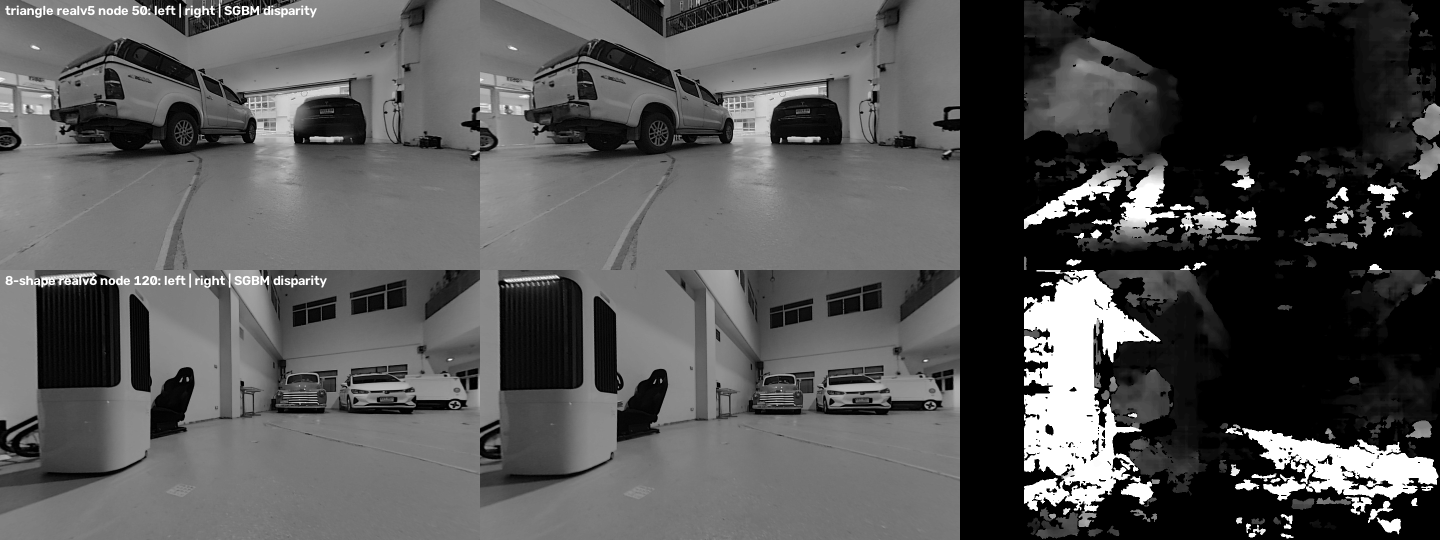
\includegraphics[width=\textwidth]{rtab/rtab_real_stereo_quality_realv5_vs_realv6.png}
\caption{Stored left and right images and the SGBM disparity of one node from
the 28~October database (top) and the 31~October database built with the same
calibration (bottom). The lower pair is vertically misaligned by about
\SI{1.2}{\pixel}, and the disparity map degrades into streaks.}
\label{fig:rtab-real-quality}
\end{figure}

\begin{figure}[htbp]
\centering
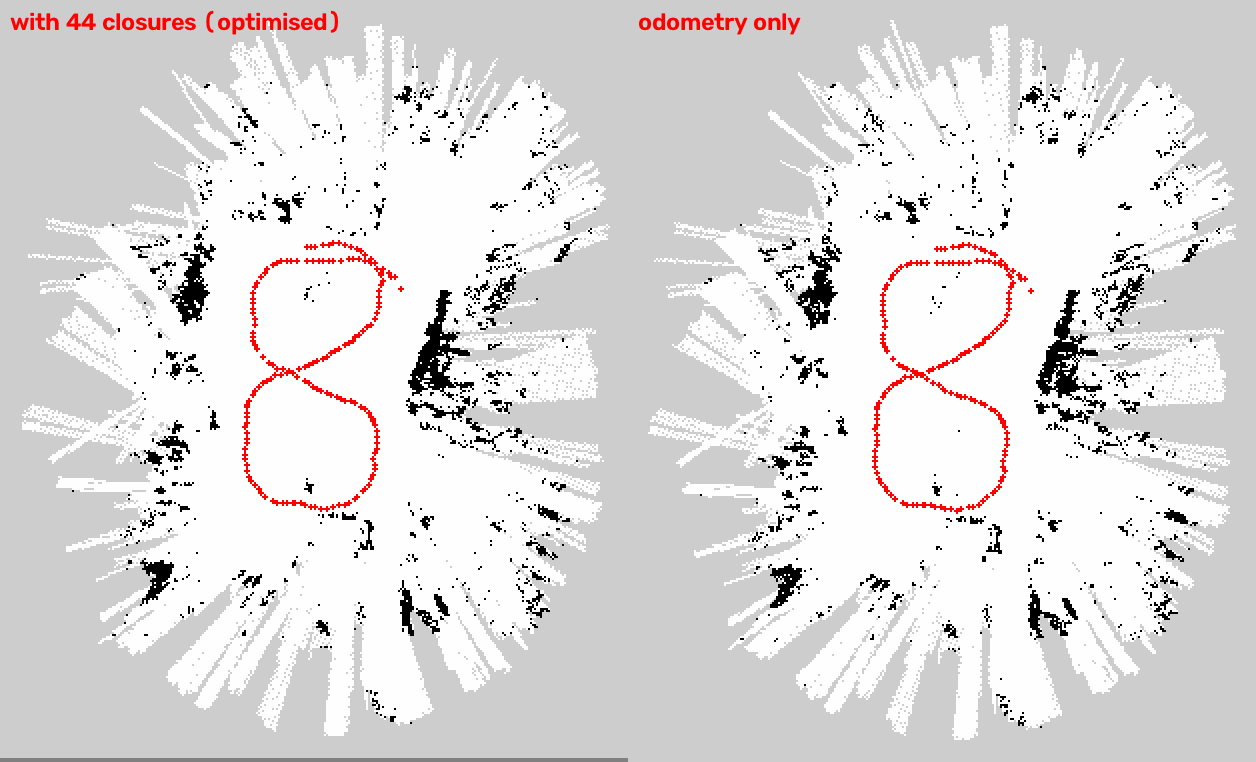
\includegraphics[width=\textwidth]{rtab/rtab_realv6_grid_closures_vs_odometry.png}
\caption{The 31~October grid exported with its 44 accepted closures (left) and
from odometry alone (right); node poses in red. The two are the same map, so
the closures are not what smeared it.}
\label{fig:rtab-realv6-closures}
\end{figure}

A self-calibration from the bag restores realv6 to the alignment realv5 has
(\cref{tab:rtab-epi}, last two rows), and the rebuilt map shows wall lines and
object outlines again (\cref{fig:rtab-realv6-selfcal}).
\repo{script/stereo_selfcal.py} recovers the rotation and the baseline
direction from an essential matrix over fisheye-undistorted matches, with the
baseline length copied from a reference file. On realv5 it lands within
\SI{0.2}{\degree} of the chequerboard rotation, which validates the method. The result is kept as
\repo{camera_parameters_311026_selfcal/} with a shim configuration in
\repo{vins_fusion_ros2/config/wil_311026_selfcal/}; the live \repo{config/wil}
is unchanged. \flag{A chequerboard calibration of the current mount is still
required: the self-calibration leaves a vertical bias of about \SI{1}{\pixel}
and cannot observe the baseline length.}

\begin{figure}[htbp]
\centering
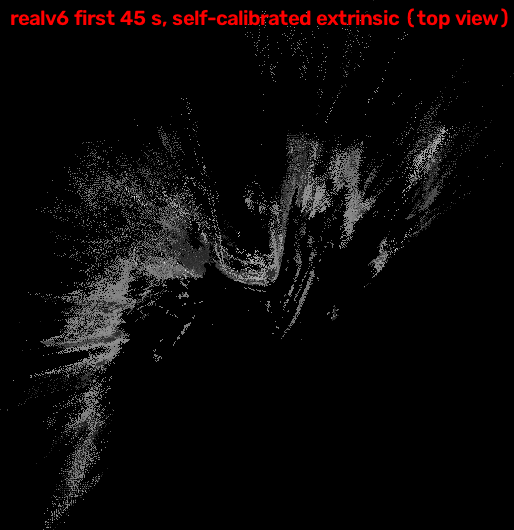
\includegraphics[width=0.6\textwidth]{rtab/rtab_realv6_selfcal_cloud_top.png}
\caption{Top view of the dense cloud from the first \SI{45}{\second} of the
31~October recording rebuilt with the self-calibrated extrinsic
(36 nodes). Structure returns; residual ray streaks remain.}
\label{fig:rtab-realv6-selfcal}
\end{figure}

\Cref{tab:rtab-depth} is the measured depth noise of the rectified pair, which
fixes the range settings: a plane fitted to the floor points of several
nodes, median distance of the points from that plane per range bin. At
\repo{rect_scale} 0.5 the depth is grid-cell accurate to about
\SI{1.5}{\metre} and within the \SI{25}{\centi\metre} scoring tolerance to
about \SIrange{3}{4}{\metre}. \repo{grid_range_max} is therefore
\SI{3}{\metre} for real-rig maps, against \SI{10}{\metre} in simulation; a
range limit for viewing the cloud is set in the viewer or the export tool and
does not touch the database.

\begin{table}[htbp]
\centering
\caption{Floor-plane residual of SGBM depth per range bin on the stored
\num{960}$\times$\num{540} pairs ($f_x B = 29.9$), median over 5--8 nodes per
database.}
\label{tab:rtab-depth}
\small
\begin{tabular}{@{}lS[table-format=2.1]S[table-format=2.1]S[table-format=2.1]S[table-format=2]@{}}
\toprule
Range [\si{\metre}] & {realv5, 28~Oct [\si{\centi\metre}]} & {realv6, self-cal. [\si{\centi\metre}]} & {realv6, misrectified [\si{\centi\metre}]} & {1\,px theory [\si{\centi\metre}]} \\
\midrule
0.5 -- 1 & 0.9 & 4.1 & 3.3 & 2 \\
1 -- 1.5 & 2.6 & 6.3 & 5.6 & 5 \\
1.5 -- 2 & 6.5 & 4.9 & 12.6 & 10 \\
2 -- 3 & 6.6 & 7.0 & 29.5 & 21 \\
3 -- 4 & 13.8 & 13.4 & 32.6 & 41 \\
4 -- 6 & 60.8 & 24.6 & 72.2 & 84 \\
\bottomrule
\end{tabular}
\end{table}

\subsection{Real recordings and databases}

\Cref{tab:rtab-real-data} registers the two real recordings that reached
RTAB-Map and the databases built from them. Neither recording has an
independent ground truth, so these databases carry node and link counts and
the calibration check, not a map-quality score. \Cref{fig:rtab-realv5-grid}
is the 28~October grid.

\begin{table}[htbp]
\centering
\caption{Real recordings and RTAB-Map databases at the cutoff. Loop closures
are RTAB-Map's accepted global and local-space links.}
\label{tab:rtab-real-data}
\small
\begin{tabular}{@{}p{3.8cm}p{3.2cm}p{3.2cm}p{4.9cm}@{}}
\toprule
Recording & Content & ORB run replayed & Databases \\
\midrule
\repo{dataset_realv5_000}, 28~Oct 15:31, \SI{134.6}{\second}, 4038 pairs at \SI{30}{\hertz}, mount of the 28~Oct calibration & triangular route past parked cars; \repo{/clock} recorded; no \repo{camera_info}, TF or ground truth & \repo{realv5_imu_cbgroup_reliable_r05_newIMU_TO_CAM_TF} (1366 rows, no reset after the transient) & \repo{map/real/real.db}: 87 nodes, 2 trivial start closures, stored pairs \SIrange{79}{87}{\percent} on-line; cars identifiable \\
\repo{dataset_realv6_000}, 31~Oct 19:00, \SI{220}{\second}, 6601 pairs, mount moved after 28~Oct & figure-of-eight in open hall & \repo{dataset_realv6_000/loopclosing_rate1} (3083 rows, ORB loop closing on, 0 closures fired) & \repo{map/real_311026_rate05/}: 168 nodes, 1 closure; \repo{map/real_311026_rate05_lc/}: 189 nodes, 34 + 10 closures; both \SIrange{7}{22}{\percent} on-line (unusable); self-calibrated rebuild of the first \SI{45}{\second}: 36 nodes, \SI{84}{\percent} \\
\bottomrule
\end{tabular}
\end{table}

\begin{figure}[htbp]
\centering
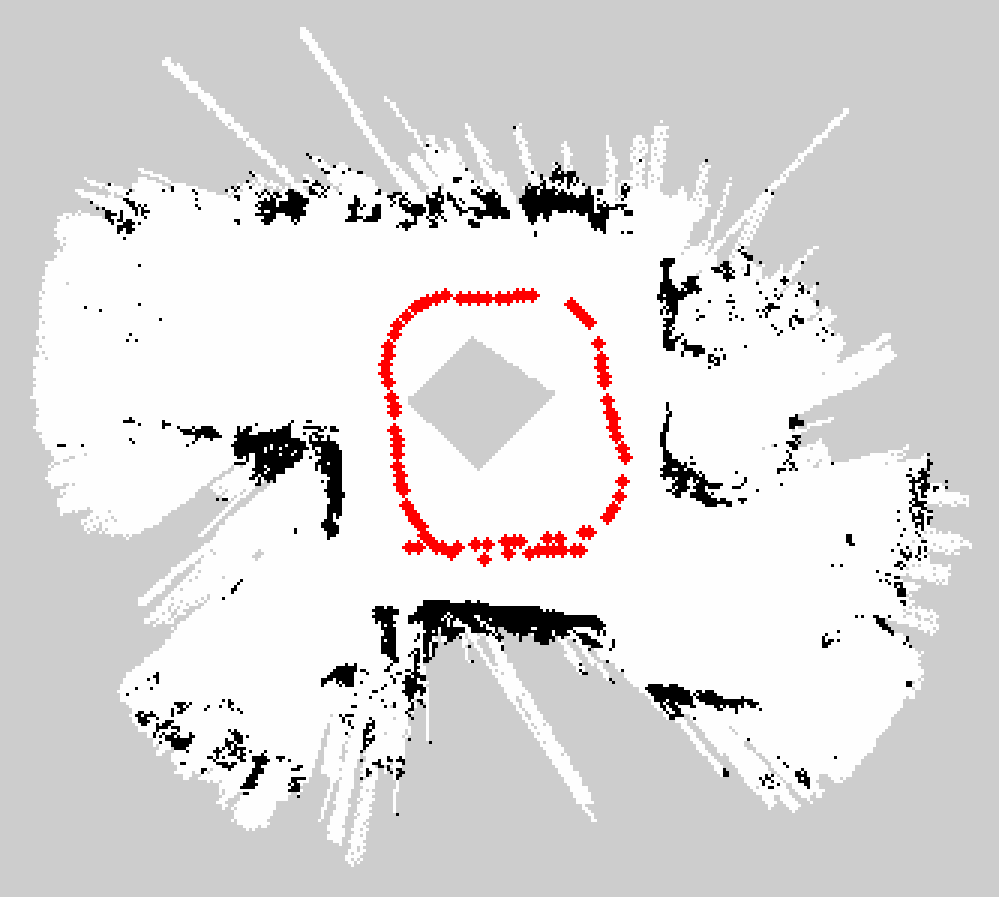
\includegraphics[width=0.55\textwidth]{rtab/rtab_realv5_grid_real_db.png}
\caption{Occupancy grid of \repoc{map/real/real.db} (28~October, 87 nodes,
\SI{5}{\centi\metre} cells, \repoc{grid_range_max} 6) with node poses in red.
Walls and parked cars appear as occupied cells; the radial streaks are
ray-traced free space from far stereo points, which the \SI{3}{\metre} range
limit of \cref{tab:rtab-depth} removes.}
\label{fig:rtab-realv5-grid}
\end{figure}

\subsection{Failure signatures}

A database with zero nodes means the input chain is dead, and the console
says where. \Cref{tab:rtab-fail} lists the signatures met while bringing the
real-rig path up, in the order to check them. A database with nodes but
no grid points instead at a grid or base-frame setting.

\begin{table}[htbp]
\centering
\caption{Zero-node failures of the real-rig chain and their signatures.}
\label{tab:rtab-fail}
\small
\begin{tabular}{@{}p{4.2cm}p{4.6cm}p{5.6cm}@{}}
\toprule
Cause & Console signature & Fix in place \\
\midrule
Shim exits at start-up: \repo{hfov_deg:=110} parsed as an integer against a double parameter & Python traceback in the launch output within \SI{2}{\second}; RTAB-Map idle & launch hands floats; shim declares the parameter dynamically typed \\
Frames before the first odometry transform & ``Did not receive data since 5 seconds'' alternating with one ``extrapolation into the past'' every \SI{10}{\second} & replay holds the first kept pose from clock start (\repo{hold_before_start}) \\
Orphaned shim from an earlier run publishing the same topics & ``Messages \ldots arrived out of order''; per-pair time ten times normal & \repo{ps -eo pid,lstart,args | grep shim} before every run; start test processes in their own session \\
Thermal throttling & RTAB-Map update \SIrange{4}{5}{\second}; then as above & start cool; bag rate 0.5 \\
\bottomrule
\end{tabular}
\end{table}

\subsection{Open items}

\begin{itemize}
\item \flag{IMU height above the floor}: measure once; it is the only
  unmeasured number in the real-rig chain.
\item \flag{Chequerboard calibration of the current mount}, then a check of
  the next recording with \repo{script/stereo_selfcal.py} before any map is
  built. Calibrate first, record second.
\item The real ORB-SLAM3 configuration carries \repo{loopClosing: 1}; set it
  to 0 for a mapping run, as in simulation, and back to 1 to load an Atlas.
\item No real-site ground truth: map quality on the real rig can only be
  assessed by the calibration check, the node and link counts and visual
  inspection until an independent reference exists.
\item The real-rig mapping bags are the ones ORB-SLAM3 was evaluated on;
  localize and extend modes have not been run on a real database.
\end{itemize}

% =====================================================================
\section{Reporting rules}
\label{sec:rtab-rules}

\begin{itemize}
\item Launch and shim: \repo{rtabmap_ros/rtab_sim.launch.py} and
  \repo{rtabmap_ros/rtab_camera_shim.py}; replay
  \repo{script/gt_tf_publisher.py}; calibration check
  \repo{script/stereo_selfcal.py}. Superproject \repo{23c6c0b}; the
  \repo{rtabmap_ros} fork at \repo{d18dc87} with the 26~October to 2~November
  changes to these files uncommitted at the cutoff.
\item Simulation measurements (\cref{tab:rtab-measured}, \cref{tab:rtab-sim-run}):
  \repo{rtabmap_ros/MEMORY_CLAUDE/README.md} Sections~5, 6, 6c, 7 and 7c; the
  ORB loop-closing A/B in \repo{output/compare/simulation/lc-mapping-ab/}.
\item Real-rig measurements (\cref{tab:rtab-hfov,tab:rtab-real-compute,tab:rtab-epi,tab:rtab-depth}):
  the same record, Section~7d; figures and their data under
  \repo{output/compare/real/rtab-config/}.
\item Databases: \repo{map/real/real.db}, \repo{map/real_311026_rate05/},
  \repo{map/real_311026_rate05_lc/}; the self-calibrated rebuild was a
  \SI{45}{\second} verification segment and is not kept as a map.
\item Real recordings:\\
  \repo{/media/ambushee/32E4AAB1E4AA772F/dataset_realv5_000} and
  \repo{dataset/dataset_realv6_000};\\
  ORB runs under \repo{output/output_orb/real/}.
\end{itemize}

\begin{thebibliography}{9}
\bibitem{labbe2019}
Labb\'e, M. and Michaud, F., 2019, ``RTAB-Map as an Open-Source Lidar and Visual Simultaneous Localization and Mapping Library for Large-Scale and Long-Term Online Operation,'' \textbf{Journal of Field Robotics}, Vol.~36, No.~2, pp.~416--446.
\bibitem{campos2021}
Campos, C., Elvira, R., G\'omez Rodr\'iguez, J.J., Montiel, J.M.M. and Tard\'os, J.D., 2021, ``ORB-SLAM3: An Accurate Open-Source Library for Visual, Visual-Inertial, and Multi-Map SLAM,'' \textbf{IEEE Transactions on Robotics}, Vol.~37, No.~6, pp.~1874--1890.
\bibitem{qin2018vins}
Qin, T., Li, P. and Shen, S., 2018, ``VINS-Mono: A Robust and Versatile Monocular Visual-Inertial State Estimator,'' \textbf{IEEE Transactions on Robotics}, Vol.~34, No.~4, pp.~1004--1020.
\bibitem{hirschmuller2008}
Hirschm\"uller, H., 2008, ``Stereo Processing by Semiglobal Matching and Mutual Information,'' \textbf{IEEE Transactions on Pattern Analysis and Machine Intelligence}, Vol.~30, No.~2, pp.~328--341.
\bibitem{kannala2006}
Kannala, J. and Brandt, S.S., 2006, ``A Generic Camera Model and Calibration Method for Conventional, Wide-Angle, and Fish-Eye Lenses,'' \textbf{IEEE Transactions on Pattern Analysis and Machine Intelligence}, Vol.~28, No.~8, pp.~1335--1340.
\end{thebibliography}
\end{document}
